\documentclass[11pt]{article}
\usepackage[margin=1in]{geometry}
\usepackage{booktabs}
\usepackage{microtype}
\usepackage{enumitem}
\usepackage[hidelinks]{hyperref}
\usepackage{titlesec}
\usepackage{pgfplots}
\pgfplotsset{compat=1.18}
\titlespacing*{\section}{0pt}{1.0em}{0.35em}
\titlespacing*{\subsection}{0pt}{0.6em}{0.25em}
\setlist{nosep,leftmargin=1.4em}
\newcommand{\code}[1]{\texttt{\small #1}}

\title{\vspace{-1.6em}A Local ReAct Coding Agent with Hidden-Test Evaluation}
\author{Vincent Le\\[-0.2em]
\small Math/Stat 361 Research, Knox College \quad\textbar\quad Advisor: Prof.\ Andrew Leahy}
\date{}

\begin{document}
\maketitle
\vspace{-2.2em}

\begin{abstract}
\noindent
I built a coding agent from scratch around a local Qwen3-14B model~\cite{qwen3} served by
vLLM~\cite{vllm}. The agent uses a standard ReAct loop~\cite{react}: the model sees a goal, a message
history, and tool schemas, then either calls tools or replies in text. It has eleven tools for file
I/O, search, shell and Python execution, subagent delegation, and explicit completion, and every file
path goes through a \code{\_safe\_path} sandbox that confines it to a workspace. I do not claim it beats
Claude or Codex. It is a small, transparent agent I can explain line by line. I evaluated it on 627
tasks with hidden tests. While hardening the project I found a leak in my own MBPP conversion script:
about 93\% of MBPP tasks exposed 2 of the 3 graded asserts to the agent, which had inflated an earlier
score of 79.9\%. After regenerating those tasks as spec-only prompts, the real score was 67.3\%
(422/627, 95\% Wilson confidence interval 64-71\%). I also reproduced the SkillOpt method of Yang et
al.~\cite{skillopt}, which optimizes a natural-language skill document while the model weights stay
frozen. On 84 test tasks the empty, seed, and optimized arms scored 0.786, 0.738, and 0.774,
exact-binomial McNemar gave $p \ge 0.29$ for every pair, and re-running the empty arm flipped about 6
of 84 tasks, so I treat that result as inconclusive.
\end{abstract}

\section{Introduction}
I wanted a coding agent I could inspect without guessing what a framework was doing. The target was
simple: take a natural-language task, operate on a local repository, edit files, run tests, and stop when
the task is done. The model was a local Qwen3-14B~\cite{qwen3}, served through vLLM~\cite{vllm} on one
GPU with an OpenAI-compatible endpoint. The Python code used the OpenAI SDK, vLLM, and
\code{python-dotenv}. No agent framework.

That constraint mattered. A framework would have made progress faster and probably handled some edge
cases better. It also would have hidden too much of the agent behind abstractions. This was a Math/Stat
361 research project, and the final artifact had to be something I could defend at the source-code level.
The goal was transparency, even at some cost to raw performance.

The agent uses ReAct, following Yao et al.~\cite{react}: the model alternates between reasoning through a
task and acting through tools. That idea is not new. Claude, Codex, and similar systems use tool-calling
loops with far better engineering around them. My system does not beat them and I do not claim it does.
The question is narrower: how far does a small local implementation get, and what breaks when you evaluate
it carefully?

The answer is mixed, and the interesting part is the second half of that question. The most common failure
was boring: the model answered in prose without calling a tool, on 66 of 627 tasks. The more important
finding was an evaluation leak I had built myself, which had made an earlier benchmark result look much
better than the system deserved. A result can look stable while a dataset pipeline is quietly leaking
information. Hidden tests and a validation gate guard against that, and a second reader caught what I had
missed.

\section{System}
The core function is \code{run\_agent(goal, workspace)}. Each iteration sends the current message history
plus the tool schemas to the local endpoint. The model returns either plain text or \code{tool\_calls}. On
tool calls, the agent executes each one, appends the result to the history as a \code{role="tool"}
message, and loops. The cap is 15 iterations.

One implementation detail became load-bearing. When the model returns an assistant message with
\code{tool\_calls}, that message has to be stored in the history verbatim. If it is not, the next request
references tool calls that no longer exist and the API rejects it with a 400. I hit this because the
message history is not a transcript for humans. It is part of the protocol.

The client uses an explicit 120-second timeout and one retry, instead of the SDK's much longer default. A
local model on a shared GPU can stall long enough to make debugging unclear, and one stuck call could
otherwise hang a whole turn. One retry tolerates a transient failure without hiding repeated ones behind
long waits. Empty responses and API errors are caught and recorded as a finish reason rather than
crashing the run.

\subsection{The eleven tools}
There are eleven tools: \code{read\_file}, \code{write\_file}, \code{apply\_patch}, \code{multi\_edit}
(file I/O); \code{list\_dir}, \code{glob\_files}, \code{grep\_files} (discovery); \code{run\_bash},
\code{run\_python} (execution); \code{spawn\_subagent} (delegation, in a separate process); and
\code{finish}. Models calling external tools in a loop is a well-studied pattern~\cite{toolformer}. The
file tools here are deliberately basic. Two of the edit tools are careful by construction:
\code{apply\_patch} refuses to apply unless its target text matches exactly once, and \code{multi\_edit}
validates every edit before writing any of them, so a bad edit never leaves a file half-written.

I made \code{finish} a tool because plain text is ambiguous. If the model says ``done'' in prose, that
might be a final answer or it might be commentary, and the runtime needs a clean signal. In this project,
replying in prose without a tool call does not end the task. The agent either calls tools, calls
\code{finish}, or runs out of iterations.

\subsection{The sandbox}
Every file path goes through one function, \code{\_safe\_path(path, workspace)}. It resolves \code{..},
turns the path into a real location, follows symlinks, and rejects anything that escapes the workspace.
The model never sees the \code{workspace} argument. It can ask to read \code{src/main.py}, but it cannot
choose the root that path is resolved against; the runtime passes that root. This is not a complete
security sandbox. \code{run\_bash} and \code{run\_python} can still execute arbitrary code, so they stay
dangerous tools. The file sandbox solves one narrower problem: file operations should not read or write
outside the assigned repository.

The loop is verbose on purpose. The runtime logs each model call, each tool invocation, each tool result,
and the model's reasoning when it is available. That is partly for debugging and mostly for studying the
agent. A silent agent that changes a file and reports only ``success'' destroys the evidence trail, and
the trail was the point.

\section{Evaluation and the Leak}
The benchmark has 627 tasks: 163 from HumanEval+~\cite{humaneval,evalplus}, 424 from MBPP~\cite{mbpp}, 37
hand-written hard tasks, and 3 legacy demos. It runs the agent on each task in a workspace and scores the
result with tests the agent never controls. During the run the grading tests are removed; the agent sees
only the prompt and the visible repository. After it stops, the grader restores the tests and runs them.
This matters because an agent with shell access can read anything left in the workspace. If the tests are
there, they are not hidden. A validation gate runs first: the reference solution must pass and the stub
must fail, or the task is pruned as broken. Keeping evaluation honest in this way is the same concern that
motivates contamination-free code benchmarks~\cite{livecodebench}.

The leak came from the MBPP converter. It was supposed to turn each task into a spec-only goal while
keeping the graded tests hidden. It did not. For about 93\% of the 424 MBPP tasks, it copied 2 of the 3
graded asserts straight into the prompt the agent could read. The agent still had to write code, but it
could see most of its own grader. The earlier full-benchmark score was 501 of 627, or 79.9\%, and it was
inflated.

I found it while hardening the project. I ran a multi-agent audit and cross-checked the evaluation setup
with a second model (Codex/GPT-5.5). The audit forced me to read the data path instead of staring at pass
rates, and once I looked at a generated MBPP prompt next to its hidden test, the leak was obvious. I
regenerated all 424 MBPP tasks with spec-only goals and reran the full benchmark. The corrected score was
422 of 627, or 67.3\% (95\% Wilson confidence interval 64-71\%~\cite{wilson}). HumanEval+ had never
leaked and stayed at about 79.8\%, which acted as a consistency check: if it had also collapsed I would
have suspected a broader benchmark change, but the drop stayed where the leak had been. Figure~\ref{fig:leak}
shows the before and after. The lower number is the one that fits the system I actually built.

\begin{figure}[h]
\centering
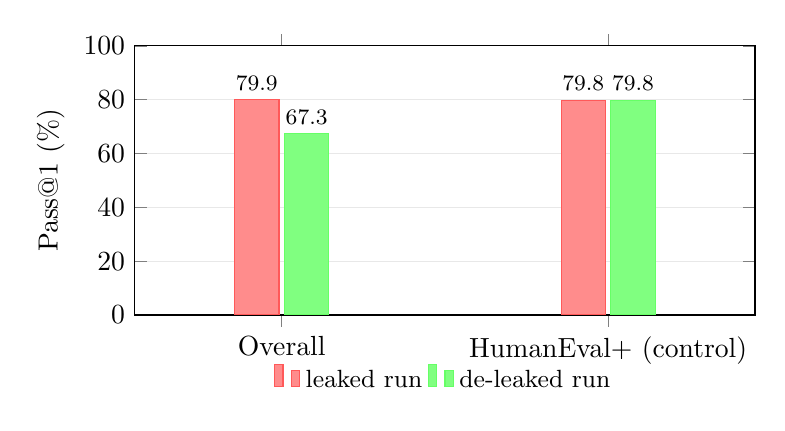
\begin{tikzpicture}
\begin{axis}[
  ybar, bar width=16pt, width=0.78\linewidth, height=5.0cm,
  ymin=0, ymax=100, ylabel={Pass@1 (\%)}, ymajorgrids, grid style={gray!18},
  symbolic x coords={Overall, {HumanEval+ (control)}},
  xtick=data, enlarge x limits=0.45,
  nodes near coords, nodes near coords style={font=\footnotesize},
  every node near coord/.append style={/pgf/number format/fixed, /pgf/number format/precision=1},
  legend style={at={(0.5,-0.16)}, anchor=north, legend columns=2, font=\small, draw=none},
]
\addplot[fill=red!45, draw=red!65] coordinates {(Overall,79.9) ({HumanEval+ (control)},79.8)};
\addplot[fill=green!50, draw=green!60] coordinates {(Overall,67.3) ({HumanEval+ (control)},79.8)};
\legend{leaked run, de-leaked run}
\end{axis}
\end{tikzpicture}
\caption{The MBPP leak, before and after the fix. The overall score fell from 79.9\% to 67.3\% once the
leaked asserts were removed. HumanEval+, which never leaked, stayed at 79.8\% in both runs and acts as a
control: the drop is confined to where the leak was.}
\label{fig:leak}
\end{figure}

\section{Results}
The corrected benchmark result is 67.3\%. Figure~\ref{fig:results} and Table~\ref{tab:results} give the
breakdown by source and by difficulty.

\begin{figure}[h]
\centering
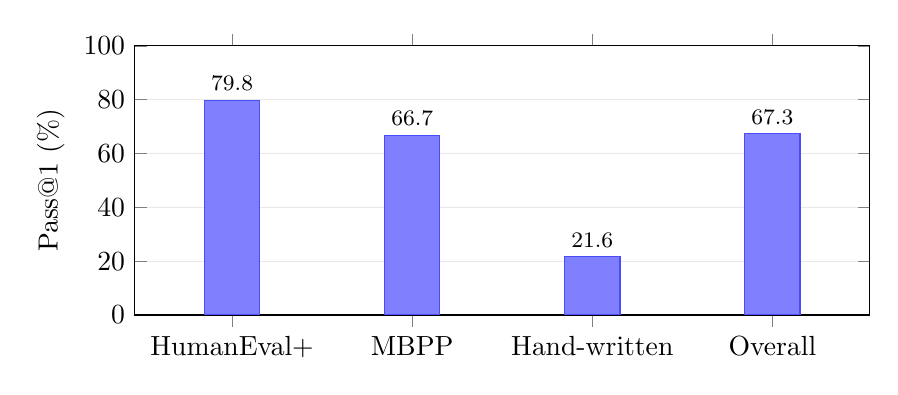
\begin{tikzpicture}
\begin{axis}[
  ybar, bar width=20pt, width=0.9\linewidth, height=5.0cm,
  ymin=0, ymax=100, ylabel={Pass@1 (\%)}, ymajorgrids, grid style={gray!18},
  symbolic x coords={HumanEval+, MBPP, Hand-written, Overall},
  xtick=data, enlarge x limits=0.18,
  nodes near coords, nodes near coords style={font=\footnotesize},
  every node near coord/.append style={/pgf/number format/fixed, /pgf/number format/precision=1},
]
\addplot[fill=blue!50, draw=blue!70] coordinates {(HumanEval+,79.8) (MBPP,66.7) (Hand-written,21.6) (Overall,67.3)};
\end{axis}
\end{tikzpicture}
\caption{Pass@1 on the de-leaked 627-task benchmark, by task source and overall. HumanEval+ ($n{=}163$),
MBPP ($n{=}424$), hand-written hard ($n{=}37$); overall 67.3\% (422/627), 95\% Wilson confidence interval
64-71\%.}
\label{fig:results}
\end{figure}

\begin{table}[h]
\centering
\begin{tabular}{lrr}
\toprule
Source & Pass@1 & $n$ \\
\midrule
HumanEval+ (never leaked)   & 79.8\% & 163 \\
MBPP, de-leaked             & 66.7\% & 424 \\
Hand-written hard           & 21.6\% & 37 \\
\midrule
\textbf{Overall}            & \textbf{67.3\%} & \textbf{627} \\
\bottomrule
\end{tabular}
\qquad
\begin{tabular}{lr}
\toprule
Difficulty & Pass@1 \\
\midrule
Easy   & 74\% \\
Medium & 74\% \\
Hard   & 54\% \\
\bottomrule
\end{tabular}
\caption{Pass@1 on the de-leaked 627-task benchmark (overall 95\% Wilson confidence interval 64-71\%).}
\label{tab:results}
\end{table}

The spread makes sense. HumanEval+ tasks are compact function-writing problems; MBPP has more variety once
the leaked asserts are gone; the hand-written hard set was built to stress the agent. Easy and medium
landing at the same rate is not a typo. The difficulty labels are coarse, and some ``easy'' tasks hide a
trap while some ``medium'' tasks are direct once the spec points at the needed behavior.

The most common failure was \code{no\_action}: on 66 of 627 tasks the model answered in prose without
calling a tool. This is a strange failure because it is not a coding mistake. The model described what
should be done and then stopped, which is useless to the runtime, because the agent cannot fix a
repository by explaining the fix. I added a guardrail that nudges the model to act when it tries to answer
without a tool call, and that recovered most of the cases. I do not treat it as a deep algorithmic
improvement. It is closer to adding a sign that says ``use the tools.'' It still mattered, because tool use
is the one behavior the whole system depends on.

Other failures were ordinary: wrong solutions, incomplete edits, tasks that hit the 15-iteration cap, and
some that simply ran into the limits of a 14B model. One more thing showed up that is worth stating: a
single benchmark run gives one number, but the local stack is not deterministic even at temperature 0.
vLLM produces run-to-run differences, which became concrete in the SkillOpt experiment below. So the
score should be read as a measurement of this implementation under this benchmark, not as a property of
Qwen3-14B or of ReAct in general.

\section{SkillOpt}
My SkillOpt experiment reproduces the method of Yang et al.~\cite{skillopt} on my own agent and benchmark.
The idea is to keep the model weights frozen and optimize a natural-language \emph{skill document} that is
prepended to the prompt. An optimizer edits it with a few bounded operations (adding, removing, or
replacing text), and a validation gate keeps a candidate only if it scores higher on a held-out split. The
model is never fine-tuned. This belongs to a line of work on optimizing text and prompts instead of
weights, including OPRO~\cite{opro}, TextGrad~\cite{textgrad}, and GEPA~\cite{gepa}, and it is close to
Voyager~\cite{voyager}, which stores and reuses skills in an agent. My implementation is a small port of
the published method's core; I deferred its larger components (a meta-skill optimizer, hierarchical
merging, an automatic learning rate) and ran it at small scale.

I evaluated three skill documents on a held-out test split of 84 tasks (Table~\ref{tab:skillopt},
Figure~\ref{fig:skillopt}). The optimized arm did not beat the empty arm. It beat the seed, but the gap
was small, and no pairwise exact-binomial McNemar test~\cite{mcnemar} reached significance ($p \ge 0.29$
for every pair).

\begin{table}[h]
\centering
\begin{tabular}{lrl}
\toprule
Skill document & Pass@1 (84 tasks) & vs.\ empty \\
\midrule
Empty (no skill)     & 0.786 & (baseline) \\
Seed (human-written) & 0.738 & McNemar $p = 1.00$ \\
Optimized            & 0.774 & McNemar $p = 0.45$ \\
\bottomrule
\end{tabular}
\caption{SkillOpt three-way comparison on the held-out test split.}
\label{tab:skillopt}
\end{table}

\begin{figure}[h]
\centering
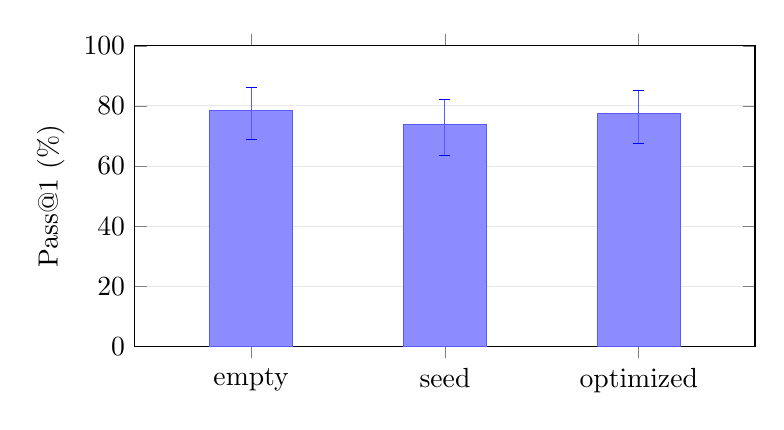
\begin{tikzpicture}
\begin{axis}[
  ybar, bar width=30pt, width=0.78\linewidth, height=5.4cm,
  ymin=0, ymax=100, ylabel={Pass@1 (\%)}, ymajorgrids, grid style={gray!18},
  symbolic x coords={empty, seed, optimized},
  xtick=data, enlarge x limits=0.3,
]
\addplot+[fill=blue!45, draw=blue!65, error bars/.cd, y dir=both, y explicit]
coordinates {
(empty,78.6)     += (0,7.4) -= (0,9.9)
(seed,73.8)      += (0,8.2) -= (0,10.3)
(optimized,77.4) += (0,7.6) -= (0,10.0)
};
\end{axis}
\end{tikzpicture}
\caption{SkillOpt arms on the 84-task held-out split, with 95\% Wilson confidence intervals: empty 78.6\%
[68.7, 86.0], seed 73.8\% [63.5, 82.0], optimized 77.4\% [67.4, 85.0]. The intervals overlap heavily, no
paired McNemar test reaches $p<0.05$, and re-running the empty arm alone flipped about 6 of 84 tasks. The
differences between arms sit inside that noise.}
\label{fig:skillopt}
\end{figure}

The run-to-run noise makes the conclusion sharper. I reran the empty arm with the same skill and settings,
and about 6 of 84 tasks flipped, roughly 7 percentage points. The gaps between arms are the same size as
the noise. A difference that size could be an optimizer effect, or it could be the inference stack moving
around. The validation set was also tiny at 12 tasks, which is small enough that an optimizer can chase
noise, and there was one scored run per arm. The clean conclusion is that the experiment is under-powered.
It does not show that skill optimization fails; it shows that this setup cannot tell. A better version
needs a larger validation set, more test tasks, several runs per arm, and tighter control over inference
nondeterminism.

\section{Limitations}
One model, served one way, on one GPU; no comparison across sizes, serving stacks, or commercial APIs.
The ReAct loop is standard, implemented from scratch but not invented here, and the agent does not exceed
Claude or Codex. The benchmark is better after the leak fix but still small: 37 hard tasks, an 84-task
SkillOpt test split, a 12-task validation set. Those catch large effects, not subtle ones. The main
conditions were scored once each, which is weak given the temperature-0 nondeterminism; a stronger study
would repeat each condition and report the variation. The sandbox is narrow: \code{\_safe\_path} protects
the file tools, but shell execution stays powerful and a real deployment would need process isolation. The
agent has no browser, no separate planner, and no memory beyond the message history and the files it
writes.

\section{What Is Mine and What Is Reused}
Reused: the ReAct pattern~\cite{react}; the benchmark tasks (HumanEval+~\cite{humaneval,evalplus} and
MBPP~\cite{mbpp}); the idea of optimizing text instead of weights~\cite{textgrad,gepa,opro}; the SkillOpt
method itself~\cite{skillopt}, which my experiment reproduces; and the notion of reusable agent skills,
which Voyager~\cite{voyager} explores for executable code. The model (Qwen3-14B~\cite{qwen3}), the serving
engine (vLLM~\cite{vllm}), and the client (OpenAI SDK, \code{python-dotenv}) are all external.

Mine: the runtime around them. That is the \code{run\_agent} loop, the tool wiring and dispatch, the
workspace sandbox, the benchmark harness with its validation gate and hidden-test scoring, the SkillOpt
experiment code (a port of the published method onto my agent), and the MBPP fix. The teaching shape is
also deliberate: the source is small, the runtime is verbose, and the examples form a ladder from a basic
chat script to a sandboxed loop, because the project had to stay explainable. The leak discovery is part
of the result. I did not plan it, but it changed the project, and the evaluation is stronger for throwing
the bad number out.

\section{Conclusion}
I built a from-scratch local coding agent on a standard ReAct loop with a small set of tools, and its
corrected hidden-test score was 67.3\% over 627 tasks. The loop itself is straightforward. The useful
technical lessons were in the details around it: store assistant tool-call messages verbatim, keep file
paths inside the workspace, give the client real timeouts, and make the model call an explicit
\code{finish}. The most useful research lesson was the MBPP leak. My first score was 79.9\% and it was
wrong, because the converter exposed graded asserts in most MBPP prompts. After fixing the tasks and
rerunning, the score dropped to 67.3\%, and HumanEval+ staying near 79.8\% helped isolate the cause. That
was a useful failure. It made the evaluation less flattering and more real. The SkillOpt result was
inconclusive: the optimized document landed near the empty baseline, the paired tests were not
significant, and the run-to-run noise was about the size of the arm gaps. The contribution is small and I
will state it plainly: a transparent local agent with a hidden-test benchmark, and an evaluation leak I
found and documented. The numbers are ones I can explain without pointing at a framework.

\begin{thebibliography}{99}
\small
\bibitem{react} S.\ Yao, J.\ Zhao, D.\ Yu, et al. ReAct: Synergizing Reasoning and Acting in Language Models. ICLR, 2023. arXiv:2210.03629.
\bibitem{reflexion} N.\ Shinn, F.\ Cassano, E.\ Berman, et al. Reflexion: Language Agents with Verbal Reinforcement Learning. NeurIPS, 2023. arXiv:2303.11366.
\bibitem{toolformer} T.\ Schick, J.\ Dwivedi-Yu, R.\ Dess\`i, et al. Toolformer: Language Models Can Teach Themselves to Use Tools. NeurIPS, 2023. arXiv:2302.04761.
\bibitem{voyager} G.\ Wang, Y.\ Xie, Y.\ Jiang, et al. Voyager: An Open-Ended Embodied Agent with Large Language Models. TMLR, 2023. arXiv:2305.16291.
\bibitem{opro} C.\ Yang, X.\ Wang, Y.\ Lu, et al. Large Language Models as Optimizers. ICLR, 2024. arXiv:2309.03409.
\bibitem{textgrad} M.\ Yuksekgonul, F.\ Bianchi, J.\ Boen, et al. TextGrad: Automatic ``Differentiation'' via Text. arXiv preprint, 2024 (published in Nature, 2025). arXiv:2406.07496.
\bibitem{gepa} L.\ A.\ Agrawal, S.\ Tan, D.\ Soylu, et al. GEPA: Reflective Prompt Evolution Can Outperform Reinforcement Learning. arXiv preprint, 2025. arXiv:2507.19457.
\bibitem{skillopt} Y.\ Yang, Z.\ Gong, W.\ Huang, et al. SkillOpt: Executive Strategy for Self-Evolving Agent Skills. arXiv preprint, 2026. arXiv:2605.23904.
\bibitem{qwen3} Qwen Team. Qwen3 Technical Report. arXiv preprint, 2025. arXiv:2505.09388.
\bibitem{vllm} W.\ Kwon, Z.\ Li, S.\ Zhuang, et al. Efficient Memory Management for Large Language Model Serving with PagedAttention. SOSP, 2023. arXiv:2309.06180.
\bibitem{humaneval} M.\ Chen, J.\ Tworek, H.\ Jun, et al. Evaluating Large Language Models Trained on Code. arXiv preprint, 2021. arXiv:2107.03374.
\bibitem{mbpp} J.\ Austin, A.\ Odena, M.\ Nye, et al. Program Synthesis with Large Language Models. arXiv preprint, 2021. arXiv:2108.07732.
\bibitem{evalplus} J.\ Liu, C.\ S.\ Xia, Y.\ Wang, et al. Is Your Code Generated by ChatGPT Really Correct? Rigorous Evaluation of Large Language Models for Code Generation. NeurIPS, 2023. arXiv:2305.01210.
\bibitem{livecodebench} N.\ Jain, K.\ Han, A.\ Gu, et al. LiveCodeBench: Holistic and Contamination Free Evaluation of Large Language Models for Code. ICLR, 2025. arXiv:2403.07974.
\bibitem{mcnemar} Q.\ McNemar. Note on the sampling error of the difference between correlated proportions or percentages. Psychometrika, 12(2):153--157, 1947.
\bibitem{wilson} E.\ B.\ Wilson. Probable Inference, the Law of Succession, and Statistical Inference. Journal of the American Statistical Association, 22(158):209--212, 1927.
\end{thebibliography}

\end{document}
